\documentclass{beamer}

\usetheme{Madrid}
\usecolortheme{default}

\usepackage{tikz}
\usetikzlibrary{fit,positioning}
\usepackage{booktabs}
\usepackage{array}
\usepackage{multirow}
\usepackage{amsmath}

\title{Research Progress}
\subtitle{Toward Byzantine Fault Tolerance in Kubernetes Control Planes}
\author{Chiharu Tomimori}
\date{\today}

\begin{document}

\begin{frame}
    \titlepage
\end{frame}

%------------------------------------------------
\begin{frame}{Research Direction}
\begin{itemize}
    \item Focus: Kubernetes as a distributed systems research topic
    \item Short-term goal: poster presentation in 5 weeks
    \item Long-term goal: study BFT for Kubernetes control planes
\end{itemize}

\vspace{0.3cm}

\begin{block}{Main Research Question}
How do crash failures and selective communication failures differently affect Kubernetes control-plane availability and convergence?
\end{block}

\vspace{0.3cm}

\begin{center}
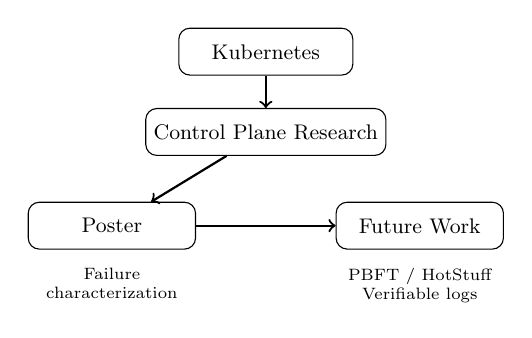
\begin{tikzpicture}[scale=0.85, every node/.style={font=\small, transform shape}]
\node[draw, rounded corners, align=center, minimum width=2.6cm, minimum height=0.7cm] (k8s) at (0,2) {Kubernetes};
\node[draw, rounded corners, align=center, minimum width=3.0cm, minimum height=0.7cm] (cp) at (0,0.8) {Control Plane Research};
\node[draw, rounded corners, align=center, minimum width=2.5cm, minimum height=0.7cm] (poster) at (-2.3,-0.6) {Poster};
\node[draw, rounded corners, align=center, minimum width=2.5cm, minimum height=0.7cm] (future) at (2.3,-0.6) {Future Work};

\draw[->, thick] (k8s) -- (cp);
\draw[->, thick] (cp) -- (poster);
\draw[->, thick] (poster) -- (future);

\node[below=0.15cm of poster, align=center, font=\scriptsize] {Failure\\characterization};
\node[below=0.15cm of future, align=center, font=\scriptsize] {PBFT / HotStuff\\Verifiable logs};
\end{tikzpicture}
\end{center}
\end{frame}

%------------------------------------------------
\begin{frame}{Why This Topic?}
\begin{columns}[T]
\column{0.56\textwidth}
\begin{itemize}
    \item Kubernetes depends on the control plane to maintain cluster state.
    \item etcd stores critical data such as Deployments, ConfigMaps, and scheduling-related state.
    \item Standard etcd uses Raft, which mainly tolerates crash failures.
    \item A component may remain alive but behave abnormally:
    \begin{itemize}
        \item delay messages,
        \item drop messages,
        \item communicate only partially.
    \end{itemize}
\end{itemize}

\column{0.44\textwidth}
\begin{center}
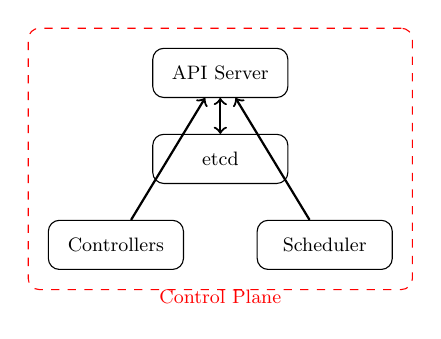
\begin{tikzpicture}[scale=0.78, every node/.style={font=\small, transform shape}]
\node[draw, rounded corners, minimum width=2.2cm, minimum height=0.8cm] (api) at (0,2.2) {API Server};
\node[draw, rounded corners, minimum width=2.2cm, minimum height=0.8cm] (etcd) at (0,0.8) {etcd};
\node[draw, rounded corners, minimum width=2.2cm, minimum height=0.8cm] (ctrl) at (-1.7,-0.6) {Controllers};
\node[draw, rounded corners, minimum width=2.2cm, minimum height=0.8cm] (sched) at (1.7,-0.6) {Scheduler};

\draw[<->, thick] (api) -- (etcd);
\draw[->, thick] (ctrl) -- (api);
\draw[->, thick] (sched) -- (api);

\node[draw=red, dashed, rounded corners, fit=(api)(etcd)(ctrl)(sched), inner sep=0.25cm] {};
\node[red, font=\small] at (0,-1.45) {Control Plane};
\end{tikzpicture}
\end{center}
\end{columns}
\end{frame}

%------------------------------------------------
\begin{frame}{What I Learned This Week}
\begin{columns}[T]
\column{0.53\textwidth}
\begin{block}{Key Understanding}
Kubernetes is not directly creating Pods from \texttt{kubectl}.  
It is a control loop system:
\begin{itemize}
    \item user request $\rightarrow$ API server
    \item desired state stored in etcd
    \item controllers reconcile the gap
    \item scheduler assigns Pods
\end{itemize}
\end{block}

\column{0.47\textwidth}
\begin{center}
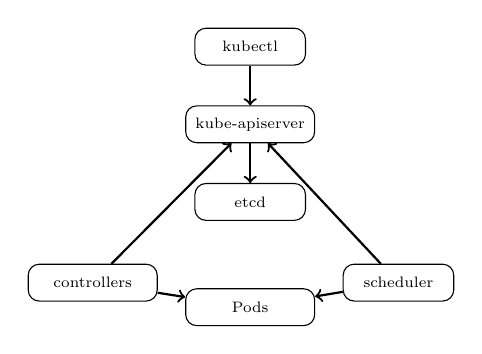
\begin{tikzpicture}[scale=0.78, node distance=0.65cm, every node/.style={font=\scriptsize, transform shape}]
\node[draw, rounded corners, minimum width=1.8cm, minimum height=0.6cm] (kubectl) {kubectl};
\node[draw, rounded corners, below=of kubectl, minimum width=2.1cm, minimum height=0.6cm] (api) {kube-apiserver};
\node[draw, rounded corners, below=of api, minimum width=1.8cm, minimum height=0.6cm] (etcd) {etcd};
\node[draw, rounded corners, below left=0.7cm and 0.6cm of etcd, minimum width=2.1cm, minimum height=0.6cm] (ctrl) {controllers};
\node[draw, rounded corners, below right=0.7cm and 0.6cm of etcd, minimum width=1.8cm, minimum height=0.6cm] (sched) {scheduler};
\node[draw, rounded corners, below=1.1cm of etcd, minimum width=2.1cm, minimum height=0.6cm] (pods) {Pods};

\draw[->, thick] (kubectl) -- (api);
\draw[->, thick] (api) -- (etcd);
\draw[->, thick] (ctrl) -- (api);
\draw[->, thick] (sched) -- (api);
\draw[->, thick] (ctrl) -- (pods);
\draw[->, thick] (sched) -- (pods);
\end{tikzpicture}
\end{center}
\end{columns}
\end{frame}

%------------------------------------------------
\begin{frame}{Deployment Creation Flow}
\begin{center}
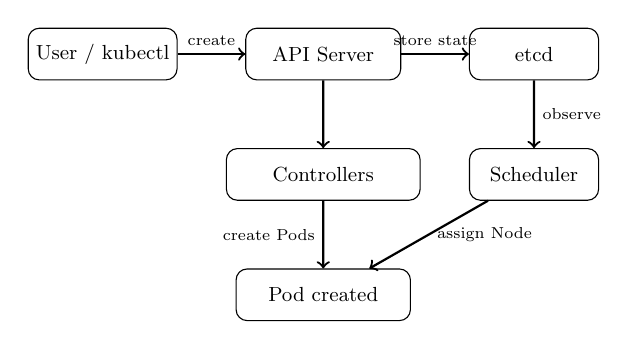
\begin{tikzpicture}[scale=0.82, every node/.style={font=\small, transform shape}, node distance=1.05cm]
\node[draw, rounded corners, minimum width=2.2cm, minimum height=0.8cm] (u) {User / kubectl};
\node[draw, rounded corners, right=of u, minimum width=2.4cm, minimum height=0.8cm] (api) {API Server};
\node[draw, rounded corners, right=of api, minimum width=2.0cm, minimum height=0.8cm] (etcd) {etcd};
\node[draw, rounded corners, below=of api, minimum width=3.0cm, minimum height=0.8cm] (ctrl) {Controllers};
\node[draw, rounded corners, below=of etcd, minimum width=2.0cm, minimum height=0.8cm] (sched) {Scheduler};
\node[draw, rounded corners, below=of ctrl, minimum width=2.7cm, minimum height=0.8cm] (pod) {Pod created};

\draw[->, thick] (u) -- node[above] {\scriptsize create} (api);
\draw[->, thick] (api) -- node[above] {\scriptsize store state} (etcd);
\draw[->, thick] (etcd) -- node[right] {\scriptsize observe} (sched);
\draw[->, thick] (api) -- (ctrl);
\draw[->, thick] (ctrl) -- node[left] {\scriptsize create Pods} (pod);
\draw[->, thick] (sched) -- node[right] {\scriptsize assign Node} (pod);
\end{tikzpicture}
\end{center}

\vspace{0.2cm}
\begin{itemize}
    \item Kubernetes stores \textbf{desired state}, not one-shot commands.
    \item State inconsistency in the control plane can affect convergence.
\end{itemize}
\end{frame}

%------------------------------------------------
\begin{frame}{Scope of the Poster Project}
\begin{table}
\centering
\small
\resizebox{\linewidth}{!}{%
\begin{tabular}{p{4.0cm} p{4.3cm} p{3.0cm}}
\toprule
\textbf{Category} & \textbf{Included} & \textbf{Excluded} \\
\midrule
Target components & etcd, API server, control-plane communication & Worker nodes \\
Faults & follower crash, leader crash, delay, selective partition & full Byzantine response forgery \\
Operations & deployment creation, scaling, ConfigMap update & large-scale workloads \\
Goal & characterize failure impact & implement PBFT/HotStuff \\
\bottomrule
\end{tabular}}
\end{table}

\vspace{0.2cm}
\begin{block}{Why this scope?}
Five weeks is too short for full BFT integration.  
So I focus on what failure behaviors matter first.
\end{block}
\end{frame}

%------------------------------------------------
\begin{frame}{Reference Paper}
\begin{center}
{\Large\bfseries On Byzantine Fault Tolerance in\\
Multi-Master Kubernetes Clusters}

\vspace{0.8cm}

{\footnotesize
G. M. Diouf, H. Elbiaze, and W. Jaafar\\
\textit{Future Generation Computer Systems}, vol. 109, pp. 407--419, 2020.}
\end{center}
\end{frame}

%------------------------------------------------
\begin{frame}{Related Work Positioning: KmMR}
\begin{block}{KmMR}
\begin{itemize}
    \item Byzantine fault tolerance for multi-master Kubernetes
    \item Uses BFT-SMaRt
    \item Proposes a BFT-based solution
\end{itemize}
\end{block}

\begin{table}
\centering
\scriptsize
\resizebox{\linewidth}{!}{%
\begin{tabular}{p{2.4cm} p{2.1cm} p{3.0cm}}
\toprule
\textbf{Aspect} & \textbf{KmMR} & \textbf{My Work} \\
\midrule
Goal & BFT solution & characterize failures \\
System & modified K8s & standard K8s \\
Method & BFT-SMaRt & fault injection \\
Output & solution perf. & problem understanding \\
\bottomrule
\end{tabular}}
\end{table}

\vspace{0.3cm}
\begin{itemize}
    \item My work is a \textbf{preparatory step} toward future BFT integration.
\end{itemize}
\end{frame}

%------------------------------------------------
\begin{frame}{Planned Fault Scenarios}
\begin{table}
\centering
\small
\begin{tabular}{p{1.5cm} p{4.2cm} p{4.5cm}}
\toprule
\textbf{ID} & \textbf{Scenario} & \textbf{Observation} \\
\midrule
F0 & Normal operation & baseline latency and convergence \\
F1 & etcd follower crash & whether service continues correctly \\
F2 & etcd leader crash & failover and recovery time \\
F3 & Network delay & API latency and convergence impact \\
F4 & Selective partition & partial communication without full stop \\
\bottomrule
\end{tabular}
\end{table}

\vspace{0.25cm}
\begin{center}
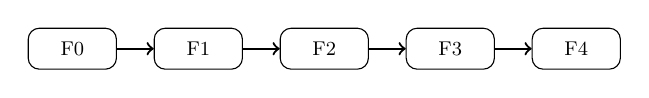
\begin{tikzpicture}[scale=0.8, every node/.style={font=\small, transform shape}]
\node[draw, rounded corners, minimum width=1.4cm, minimum height=0.65cm] (f0) at (0,0) {F0};
\node[draw, rounded corners, minimum width=1.4cm, minimum height=0.65cm] (f1) at (2,0) {F1};
\node[draw, rounded corners, minimum width=1.4cm, minimum height=0.65cm] (f2) at (4,0) {F2};
\node[draw, rounded corners, minimum width=1.4cm, minimum height=0.65cm] (f3) at (6,0) {F3};
\node[draw, rounded corners, minimum width=1.4cm, minimum height=0.65cm] (f4) at (8,0) {F4};
\draw[->, thick] (f0) -- (f1);
\draw[->, thick] (f1) -- (f2);
\draw[->, thick] (f2) -- (f3);
\draw[->, thick] (f3) -- (f4);
\end{tikzpicture}
\end{center}
\end{frame}

%------------------------------------------------
\begin{frame}{Evaluation Metrics}
\begin{columns}[T]
\column{0.55\textwidth}
\begin{itemize}
    \item \textbf{Success rate}: does the operation complete?
    \item \textbf{Latency}: how long does it take?
    \item \textbf{Convergence time}: when do desired Pods become ready?
    \item \textbf{Recovery time}: how long after a failure?
    \item \textbf{Detection}: does Kubernetes notice the abnormal condition?
\end{itemize}

\column{0.45\textwidth}
\begin{center}
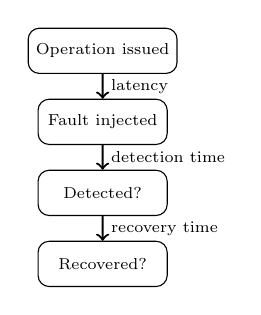
\begin{tikzpicture}[scale=0.82, every node/.style={font=\scriptsize, transform shape}]
\node[draw, rounded corners, minimum width=2.0cm, minimum height=0.7cm] (op) at (0,2.5) {Operation issued};
\node[draw, rounded corners, minimum width=2.0cm, minimum height=0.7cm] (fault) at (0,1.4) {Fault injected};
\node[draw, rounded corners, minimum width=2.0cm, minimum height=0.7cm] (detect) at (0,0.3) {Detected?};
\node[draw, rounded corners, minimum width=2.0cm, minimum height=0.7cm] (recover) at (0,-0.8) {Recovered?};

\draw[->, thick] (op) -- node[right] {latency} (fault);
\draw[->, thick] (fault) -- node[right] {detection time} (detect);
\draw[->, thick] (detect) -- node[right] {recovery time} (recover);
\end{tikzpicture}
\end{center}
\end{columns}
\end{frame}

%------------------------------------------------
\begin{frame}{5-Week Plan}
\begin{table}
\centering
\small
\begin{tabular}{p{1.2cm} p{9.4cm}}
\toprule
\textbf{Week} & \textbf{Plan} \\
\midrule
1 & Fix scope, understand control plane flow, read KmMR, prepare environment \\
2 & Baseline measurements and crash-fault experiments \\
3 & Delay and selective communication-failure experiments \\
4 & Analyze results and connect them to PBFT / HotStuff motivation \\
5 & Finalize poster, figures, and presentation story \\
\bottomrule
\end{tabular}
\end{table}

\vspace{0.3cm}
\begin{block}{This Week's Progress}
\begin{itemize}
    \item Fixed the poster scope
    \item Understood the control-plane operation flow
    \item Started positioning the work against KmMR
\end{itemize}
\end{block}
\end{frame}

%------------------------------------------------
\begin{frame}{Takeaways}
\begin{itemize}
    \item Kubernetes is a \textbf{desired-state distributed control system}.
    \item etcd is central because it stores the cluster state.
    \item Crash failures and communication abnormalities are not the same.
    \item Before introducing PBFT or HotStuff, I first need to identify what kinds of failures actually hurt Kubernetes.
    \item This poster project builds the foundation for future BFT-based Kubernetes research.
\end{itemize}
\end{frame}

\end{document}
